\subsection{Évaluation et métriques}

En \gls{ml}, l'évaluation quantitative de la performance d'un modèle est une étape incontournable.
Elle permet d'obtenir des mesures objectives de la qualité du modèle.
Cela est d'autant plus important que le modèle est destiné à être déployé dans un système critique.
Pour ce faire, il faut définir des métriques qui peuvent, 
à partir des prédictions du modèle et des valeurs réelles,
fournir un nombre (où une liste de nombres) qui représente la qualité du modèle.
La \gls{mt} étant un exemple de problème de classification en grande dimension%
\footnote{
Où les classes sont les tokens du vocabulaire de la langue cible.
}~\cite{deep-nmt-survey},
les métriques utilisées sont celles de la classification.

\subsubsection{Entropie croisée}

L'entropie croisée est une mesure de la dissimilarité de deux lois de probabilité%
~\cite{Vasilev_Slater_Spacagna_Roelants_Zocca_2019}.
Pour deux lois de probabilité \(p\) et \(q\) sur le même espace probabilisable \((\Omega, \mathcal{A})\),
leur entropie croisée \(H(p, q)\) est définie par :
\begin{equation}
    \label{eq.cross-entropy}
    H(p, q) = H(p) + D_{KL}(p \parallel q)
\end{equation}
où \(H(p)\) est l'entropie de \(p\) 
et \(D_{KL}(p \parallel q)\) est la divergence de Kullback-Leibler de \(p\) par rapport à \(q\)~\cite{Bishop_2006}.
Dans le cas de lois de probabilité discrètes, l'équation~\ref{eq.cross-entropy} devient :
\begin{equation}
    \label{eq.cross-entropy-discrete}
    H(p, q) = \esp_{X \sim p} \left[ - \log q(x) \right]
    = - \sum_{x \in \Omega} p(x) \log q(x)
\end{equation}
où nous avons, par abus de notation, noté \(p(x)\) et \(q(x)\) 
les probabilités des événements \(\{x\}\) par les lois \(p\) et \(q\) respectivement.

Quand l'entropie croisée est utilisée dans le cadre d'un problème de classification,
on prend souvent comme \(p\) la loi de probabilité \emph{cible}, c'est-à-dire celle des valeurs réelles.
Dans notre cas, il s'agit de la loi du prochain token sachant la phrase source et les tokens précédents.
On prend généralement une \emph{loi de Dirac}%
\footnote{
    Pour un espace probabilisable \((\Omega, \mathcal{A})\) et \(a\in\Omega\),
    la loi de Dirac \(\delta_a: \mathcal{A} \to \{0, 1\}\) est définie par :
    \(
        \delta_a(X) = 
        \begin{cases}
            1 & \text{si } a \in X \\
            0 & \text{sinon}
        \end{cases}    
    \)
}, on parle dans ce cas d'encodage \emph{\foreignlanguage{english}{one-hot}}.
Pour la loi \(q\), la sortie du modèle (typiquement avec une fonction \(\softmax\)) est prise.
L'entropie croisée devient donc une mesure de la déviation de la sortie du modèle de la vérité terrain.
Sa minimisation est donc un objectif naturel pour l'entraînement du modèle.

\begin{figure}[htb]
    \begin{center}
        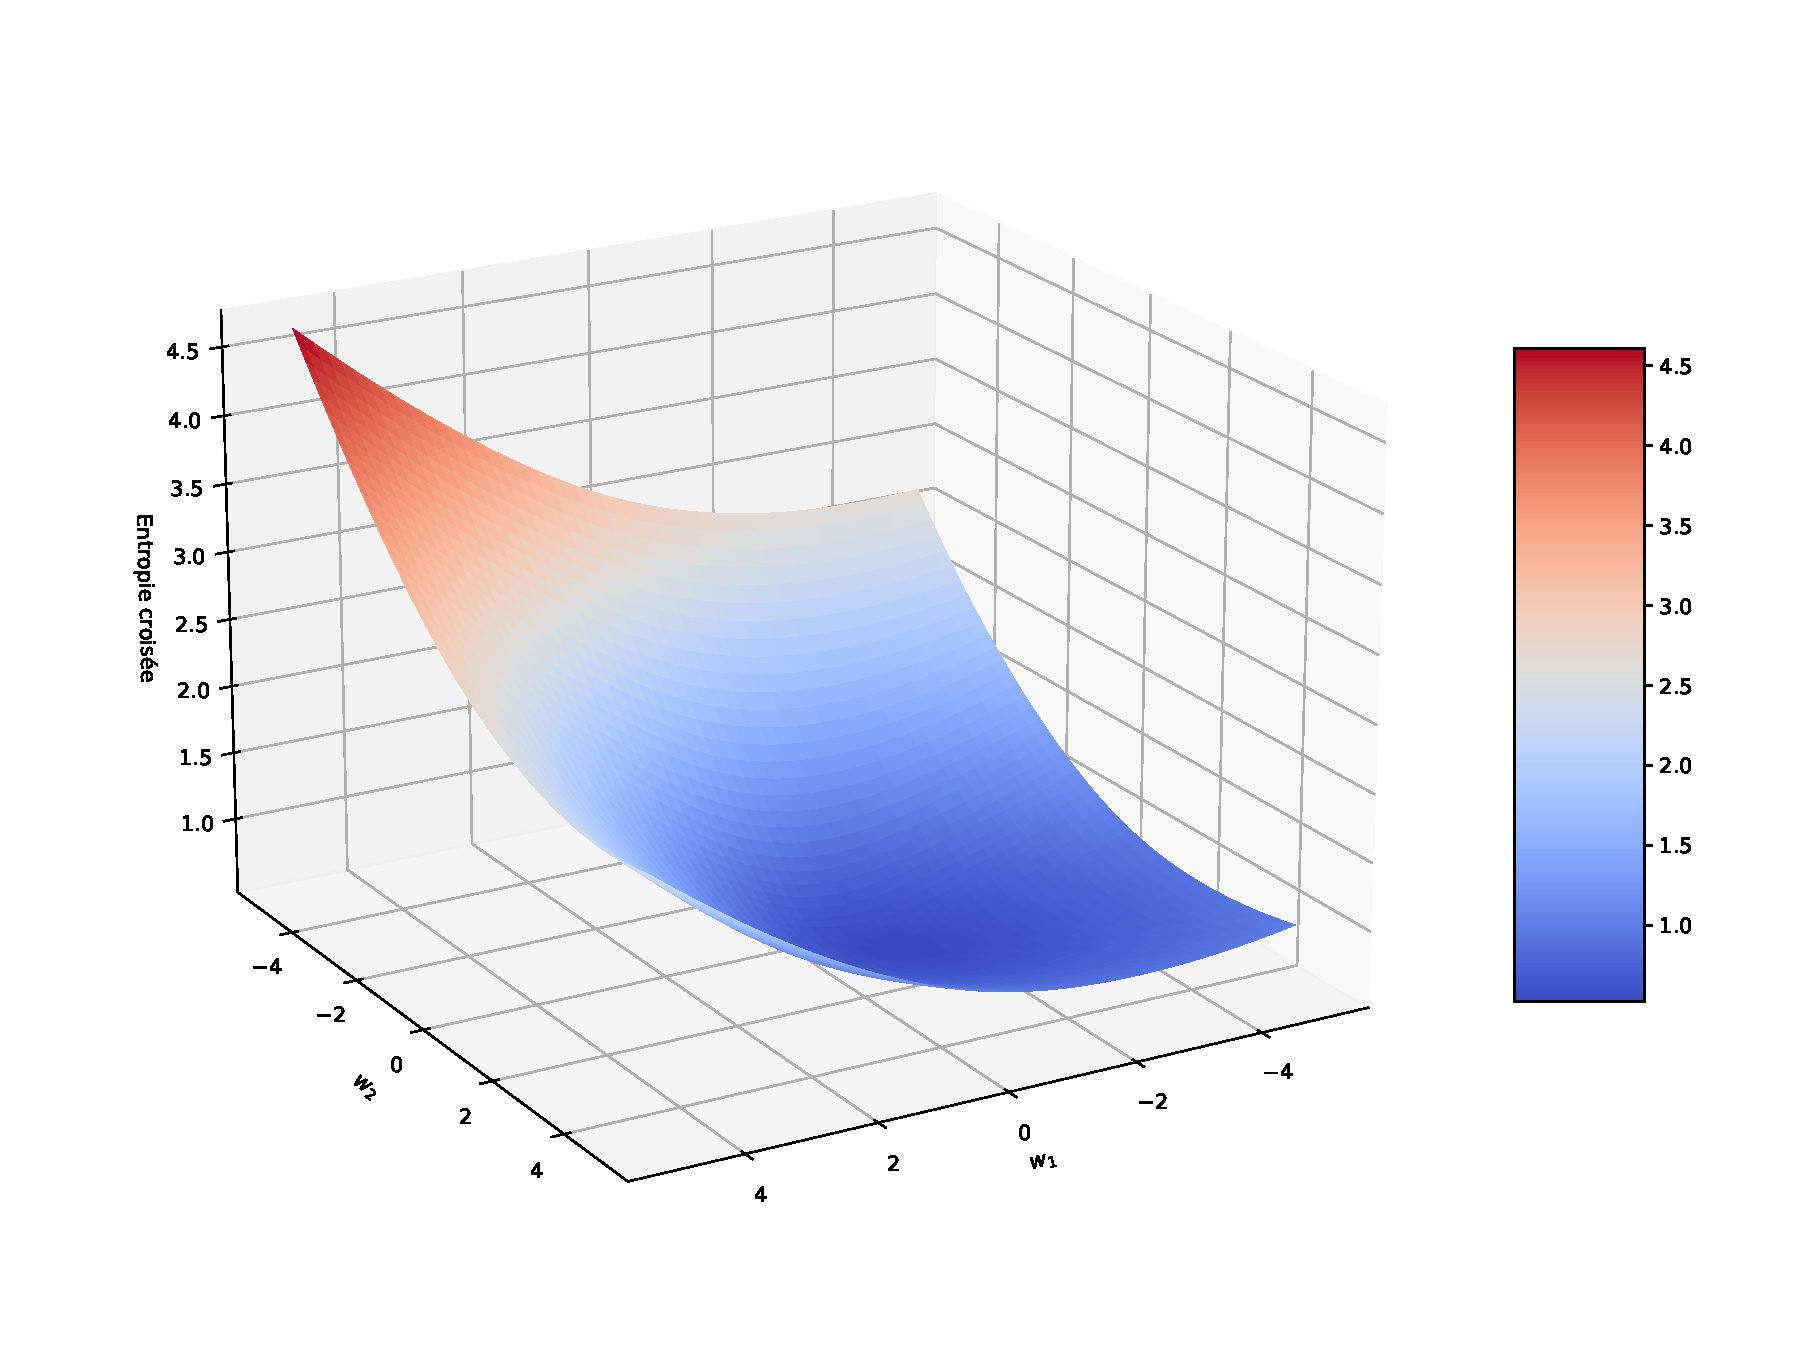
\includegraphics[width=10cm]{assets/python/cross-entropy.pdf}
    \end{center}
    \caption{Entropie croisée d'un classifieur linéaire binaire.}
    \label{fig.cross-entropy}
\end{figure}

L'entropie croisée présente un avantage important par rapport aux autres métriques de classification :
elle est \emph{dérivable} par rapport aux paramètres du modèle.
La Figure~\ref{fig.cross-entropy} l'illustre sur le cas d'un modèle de régression logistique en deux dimensions.
On y voit que la surface qui représente l'entropie croisée est lisse.
Elle est également convexe dans ce cas, mais cela n'est pas vrai pour un réseau de neurones.

Le fait d'être dérivable (contrairement à la majorité des alternatives)
rend possible sa minimisation par un algorithme de gradient comme Adam.
C'est pour cette raison que l'entropie croisée est la fonction de perte la plus utilisée en classification.
Pour cette même raison, elle est utilisée dans notre système pour l'entraînement du modèle.

Cela étant dit, l'entropie croisée a le défaut de ne pas être interprétable.
Comme elle prend ses valeurs dans l'interval \([0, +\infty]\), 
elle ne donne aucune information sur la différence relative entre deux modèles.
Elle permet de déterminer si un modèle \(\mathcal{M}\) est plus performant qu'un autre modèle \(\mathcal{M}^\prime\),
mais elle ne nous dit rien sur le degré auquel \(\mathcal{M}\) dépasse \(\mathcal{M}^\prime\).
Pour cette raison, des métriques normalisées sont nécessaires pour comparer des modèles.

\subsubsection{Exactitude, précision, rappel et mesure \(F_\beta\)}

Une façon universelle d'évaluer la performance d'un modèle de classification 
est de regarder sa \emph{matrice de confusion}.
Il s'agit d'une matrice carrée \(M\) 
dont les lignes sont indexées par les classes réelles et les colonnes par les classes prédites.
L'élément à la position \((i, j)\) de la matrice 
est le nombre d'exemples de la classe \(i\) attribués par le modèle à la classe \(j\).
Un modèle parfait à donc une matrice diagonale pour matrice de confusion.

Il est moins facile d'interpréter la matrice de confusion d'un modèle imparfait.
Pour cette raison, il est utile d'en extraire des nombres directement interprétables.
Il est possible de construire ces nombres à partir de la matrice de confusion 
en posant 3 questions assez naturelles :
\begin{enumerate}[label=(\arabic*)]
    \item Quelle est la proportion d'exemples correctement classés ? 
    C'est-à-dire, quelle est la proportion d'exemples pour lesquels 
    la classe prédite est la même que la classe réelle ?
    \item Quelle proportion des exemples de la classe \(i\) est attribuée à la classe \(i\) ?
    \item Quelle proportion des exemples attribués à la classe \(j\) est réellement de la classe \(j\) ?
\end{enumerate}

La réponse à la première question est donnée par \emph{l'exactitude} du modèle.
Il s'agit d'un nombre entre 0 et 1 qui mesure la similarité entre 
la matrice de confusion du modèle et la matrice diagonale du modèle parfait.
L'exactitude est définie par :
\begin{equation}
    \label{eq.accuracy}
    \text{exactitude} =  \frac{\tr{M}}{\text{sum}(M)} 
                      = \frac{\sum\limits_{i=1}^n M_{ii}}{\sum\limits_{i=1}^n \sum\limits_{j=1}^n M_{ij}}
\end{equation}
elle donne une mesure de la performance globale du modèle, indépendamment des classes.
Cela n'est pas toujours souhaitable,
un exemple d'un cas problématique est celui d'un modèle qui prédit toujours la classe majoritaire.
L'exactitude de ce modèle est minorée par la fréquence de cette classe.
Dans le cas où les classes sont très déséquilibrées,
un modèle sans aucune capacité à décerner les classes minoritaires peut avoir une exactitude élevée
en attribuant simplement toutes les classes à l'une des classes majoritaires.
Cela suggère un besoin de mesures spécifiques aux classes,
ce qui est ce que nous obtenons en abordant les questions (2) et (3).

Les réponses des deux questions restantes sont parfaitement symétriques (comme le sont les questions elles-mêmes).
Elles sont données respectivement par le \emph{rappel} et la \emph{précision} du modèle.
Le rappel de la classe \(i\) est défini par :
\begin{equation}
    \label{eq.recall}
    \text{rappel}_i = \frac{M_{ii}}{\sum\limits_{j=1}^n M_{ij}}
\end{equation}
il nous permet de savoir, sachant la classe d'un exemple, la probabilité que le modèle le classe correctement.
Une valeur élevée de rappel suggère que le modèle a tendance à bien identifier les éléments de la classe \(i\)
(on dit qu'il a peu de \emph{faux négatifs} pour cette classe).
La précision de la classe \(j\) est définie par :
\begin{equation}
    \label{eq.precision}
    \text{précision}_j = \frac{M_{jj}}{\sum\limits_{i=1}^n M_{ij}}
\end{equation}
elle nous permet de savoir, sachant la prédiction du modèle, la probabilité qu'elle soit correcte.
Une grande précision suggère que le modèle a tendance à ne pas attribuer la classe \(j\) à tort
(on dit qu'il a peu de \emph{faux positifs} pour cette classe).
Il est possible d'obtenir à partir de la précision et du rappel des mesures globales comme l'exactitude.
Il suffit pour cela de prendre la moyenne des précisions ou des rappels sur toutes les classes.
Cela présente l'avantage de traiter équitablement toutes les classes.

La mesure \(F_\beta\) permet d'agréger le rappel et la précision en une seule mesure
qui contient l'information sur les faux positifs et les faux négatifs.
Elle est paramétrée par un réel positif \(\beta\) 
qui peut être interprété comme le degré d'importance des faux positifs comparé aux faux négatifs.
Un \(\beta = 2\) signifie que les faux positifs sont pénalisés 2 fois plus que les faux négatifs%
~\cite{books/bu/Rijsbergen79}.
Le score \(F_\beta\) est défini comme la \emph{moyenne harmonique} de la précision et le rappel
pondérée par \(\alpha = \frac{1}{1 + \beta^2}\) :
\begin{equation}
    \label{eq.fbeta}
    F_\beta = \frac{1}{\frac{\alpha}{P} + \frac{1 - \alpha}{R}}
\end{equation}
où \(P\) et \(R\) sont respectivement la précision et le rappel du modèle.
La valeur la plus courante de \(\beta\) est 1,
on parle alors simplement de \(F_1\)-mesure.


\subsubsection{Score \glsfmtshort{bleu}}

Toutes les métriques discutées jusqu'à présent sont des métriques de classification.
Elles ne sont pas spécifiques à la tâche de traduction.
En effet, elles mesurent la performance du modèle sur le niveau des tokens individuels.
Elles nous apprennent rein sur sa performance au niveau des phrases entières.

Pour combler cette lacune, des métriques comme \gls{bleu} (voir Section~\ref{sec.nmt-transformer}) ont été conçues.
Dans notre travail, nous avons choisi de l'utiliser comme objectif 
pour le réglage des hyperparamètres pendant la validation.
Nous l'avons calculé sur les sorties du modèle avec \emph{forçage de l'enseignement}.
Cela signifie que la sortie est produite à partir de l'entrée et d'une version décalée 
d'elle-même avec un masque causal (voir Section~\ref{sec.transformers}).


